\documentclass[11pt,a4paper]{article}
\usepackage[T1]{fontenc}
\usepackage[utf8]{inputenc}
\usepackage{lmodern}
\usepackage[margin=22mm,headheight=16pt]{geometry}
\usepackage{amsmath,amssymb,graphicx,array,longtable,booktabs}
\usepackage{microtype,xcolor,hyperref,xurl,fancyhdr}
\definecolor{Navy}{HTML}{17324D}
\definecolor{Teal}{HTML}{087F8C}
\definecolor{Gold}{HTML}{B88128}
\hypersetup{colorlinks=true,linkcolor=Navy,urlcolor=Teal,bookmarksnumbered=true,hypertexnames=false}
\setlength{\parindent}{0pt}
\setlength{\parskip}{6pt}
\setlength{\emergencystretch}{4em}
\setcounter{tocdepth}{1}
\pagestyle{fancy}\fancyhf{}
\fancyfoot[R]{\small\thepage}
\fancyfoot[L]{\small\sffamily Sharif University of Technology}
\renewcommand{\headrulewidth}{0.3pt}
\makeatletter
\renewcommand\section{\@startsection{section}{1}{\z@}{-3.2ex plus -1ex minus -.2ex}{1.6ex plus .2ex}{\normalfont\Large\sffamily\bfseries\color{Navy}}}
\renewcommand\subsection{\@startsection{subsection}{2}{\z@}{-2.5ex plus -1ex minus -.2ex}{1.2ex plus .2ex}{\normalfont\large\sffamily\bfseries\color{Teal}}}
\makeatother
\fancyhead[L]{\small\sffamily\color{Navy}Sharif University of Technology}\fancyhead[R]{\small\sffamily\color{Teal}Project Assignment}\begin{document}
\begin{titlepage}\centering\vspace*{7mm}

\includegraphics[width=31mm]{assets/sharif_emblem_en.png}\par\vspace{5mm}
{\Large\sffamily\bfseries\color{Navy}SHARIF UNIVERSITY OF TECHNOLOGY\par}
\vspace{2mm}{\sffamily Department of Electrical Engineering\par}
\vspace{17mm}{\color{Teal}\rule{\linewidth}{1.4pt}}\par\vspace{6mm}
{\large\sffamily\color{Teal}PROJECT ASSIGNMENT\par}
\vspace{8mm}{\huge\sffamily\bfseries\color{Navy}Distributed Sensor Monitoring with HTTP, MQTT, SNMP, and SQLite\par}
\vspace{9mm}{\color{Gold}\rule{45mm}{1pt}}\par\vfill
\begin{minipage}{.88\linewidth}
{\sffamily\color{Teal}INSTRUCTOR / INSTRUCTORS}\par
Dr Iman Gholampour\par\vspace{7mm}
{\sffamily\color{Teal}ACADEMIC CONTEXT}\par
Embedded Systems\par\end{minipage}\vfill
\end{titlepage}
\tableofcontents\clearpage
\section{Scenario and system objective}

Act as the engineer of a hotel-monitoring system. Floors contain temperature, humidity, motion, and other environmental sensors. Each node receives and stores readings for its connected sensors. One master receives operator requests and returns the final result. Slave nodes communicate with the master and do not directly serve the operator. If the requested reading is absent locally, the request must continue to the next node until a result or a final not-found response returns through the master.

\section{General implementation and submission rules}

Use C or C+\allowbreak{}+\allowbreak{} only. Organize the six parts into separately numbered directories, each containing its own source, scripts, answers, guide, and report. Write the report from a system designer's perspective:\allowbreak{} architecture, components, communication, request/\allowbreak{}response paths, and decisions, rather than line-by-line code commentary. Include at least one architecture or data-flow diagram for each part. Every part requires a Markdown guide explaining dependencies, compilation, execution, requests, and tests. Use Makefiles. Supply a Bash build-and-run script;\allowbreak{} the original rules assign zero to a part lacking this script. Git is recommended and receives credit, although it is optional. Initialize databases from the supplied data files;\allowbreak{} evaluation files can change. Hard-coded answers or sensor values invalidate the exercise. IP addresses, ports, database locations, and execution settings must come from configuration, command-line arguments, or environment variables. AI assistance is permitted;\allowbreak{} evaluation focuses on system design, implementation correctness, executability, organization, and analysis. Provide a short final test video. Show each build/\allowbreak{}run script, requests and responses, the master/\allowbreak{}slave lookup, caching-time difference, MQTT exchange, SNMP readings, history API output, and alerts in the database. The requested video demonstrates operation and results;\allowbreak{} it should not explain internal code or architecture.

\section{Preliminary research: 10 percent}

Before implementing, explain Mongoose and how it supports a C/\allowbreak{}C+\allowbreak{}+\allowbreak{} HTTP server and API;\allowbreak{} distributed databases and several example systems;\allowbreak{} the meaning and use of an API;\allowbreak{} LAN communication among nodes;\allowbreak{} and distributed-system properties, benefits, and design challenges.

\section{Required directory organization}

Create parts 01 through 06. Parts 01, 02, and 03 each contain master, slave, and scripts directories, plus a report and README. Part 04 contains SNMP configuration and scripts. Part 05 contains the API and scripts. Part 06 contains the daemon, scripts, and service definitions. Internal organization may change when justified, but each part must remain independent and contain everything required to build, run, and test it.

\section{Part 1: base distributed database, 30 percent}

Create one master and two slaves as Ubuntu 22.04 virtual machines on the same network. Assign valid addresses and communicate by IP and port. Verify connectivity and include a network diagram. Give each node a local SQLite database and initialization script using the supplied files. Before implementation, inspect the schema and input data and explain them briefly. Implement master and slave programs. A request contains sensor type and identifier;\allowbreak{} the output is the latest recorded value. Mongoose may implement the HTTP API. Obtain addresses and ports dynamically. The operator sends requests only to the master. The master searches locally, forwards a miss to slave 1, continues to slave 2 if necessary, and returns the result. If no node contains the reading, return an appropriate not-found message. Explain whether forwarding is performed by successive nodes or coordinated by the master;\allowbreak{} do not hide a difference between the requested and implemented path. The suggested master directory contains main.c/\allowbreak{}main.cpp, Makefile, master\_\allowbreak{}init\_\allowbreak{}db.sh, and config.example;\allowbreak{} the slave has corresponding source, Makefile, slave\_\allowbreak{}init\_\allowbreak{}db.sh, and example configuration. The scripts directory contains build\_\allowbreak{}and\_\allowbreak{}run.sh and test\_\allowbreak{}requests.sh. The Markdown guide must explain dependency installation;\allowbreak{} compilation and execution of both node types;\allowbreak{} requests with curl;\allowbreak{} the database schema;\allowbreak{} topology;\allowbreak{} request/\allowbreak{}response path;\allowbreak{} HTTP security and improvements. Grading considers correct operation and responses, working automation, SQLite use, the diagram, dynamic addresses/\allowbreak{}ports, and security explanation. An optional advanced extension may manage nodes using one shared IP with different ports. Document its diagram, address/\allowbreak{}port settings, program execution, build/\allowbreak{}run script, and full Markdown instructions if implemented.

\section{Part 2: two-layer storage and caching, 20 percent}

Retain SQLite as the primary database and add a RAM-resident Memcached layer to every node. Check the cache first. Return a hit directly;\allowbreak{} on a miss, read SQLite, populate the cache, and return the reading. Explain both read and write behavior. Master and slave output must include the latest reading and response time. Supply Makefiles and Bash scripts for applications and supporting services. The suggested directories contain separate database initialization, Memcached initialization, and config.example files for each node type, plus scripts/\allowbreak{}build\_\allowbreak{}and\_\allowbreak{}run.sh and benchmark\_\allowbreak{}read.sh. Write a benchmark that reads every sensor in two rounds. The first round may miss the cache;\allowbreak{} the second should hit unless the design causes another outcome. Explain initialization, hit/\allowbreak{}miss paths, expiration or eviction, any second-round miss, measured round times, and the comparison. The guide must cover Memcached installation/\allowbreak{}startup, compilation, node execution, requests, benchmark execution, and interpretation.

\begin{figure}[!htbp]\centering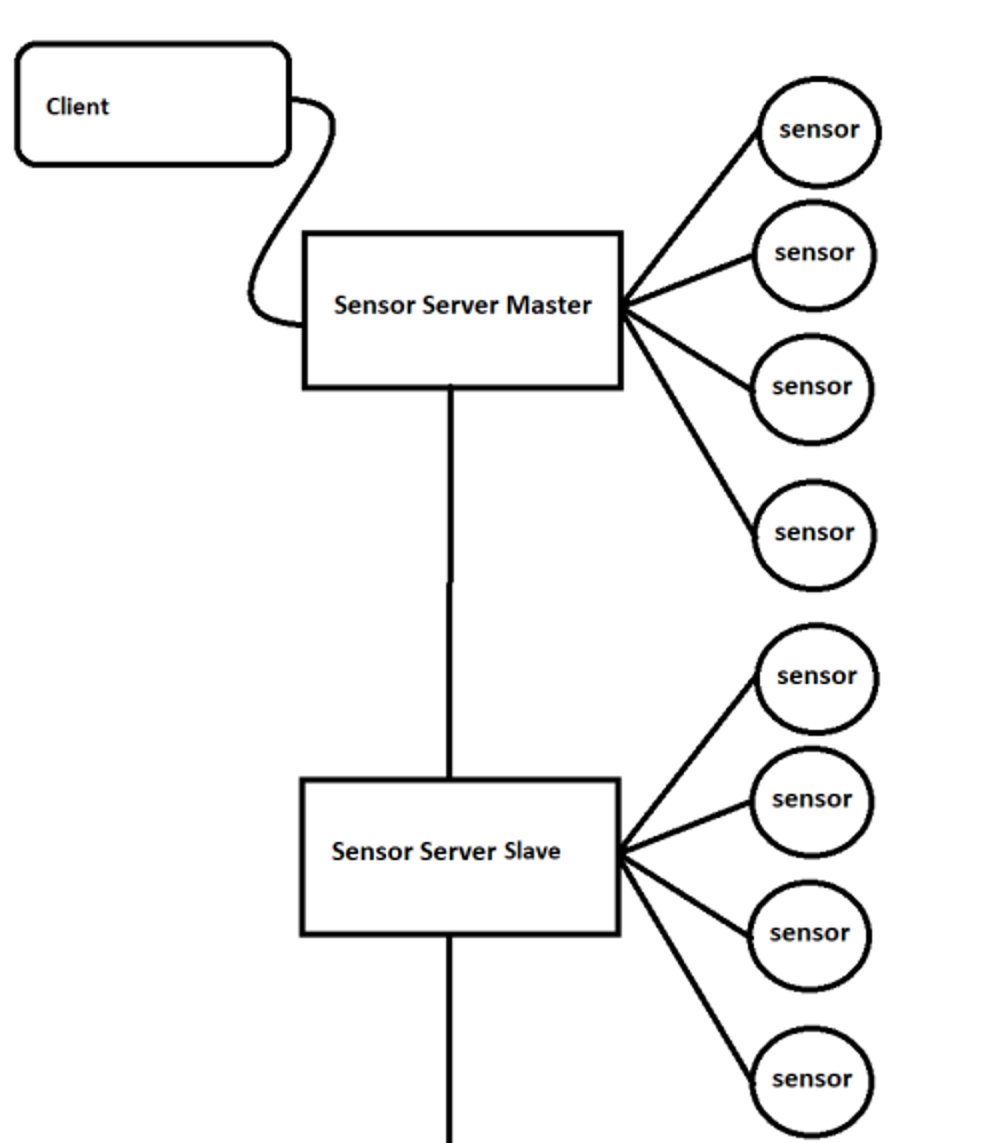
\includegraphics[width=\linewidth,height=.72\textheight,keepaspectratio]{assets/018_p002_01_panel1.png}\caption{Diagram or recorded result: Part 2: two-layer storage and caching, 20 percent. Panel 1 of 2.}\label{fig:018_p002_010}\end{figure}

\begin{figure}[!htbp]\centering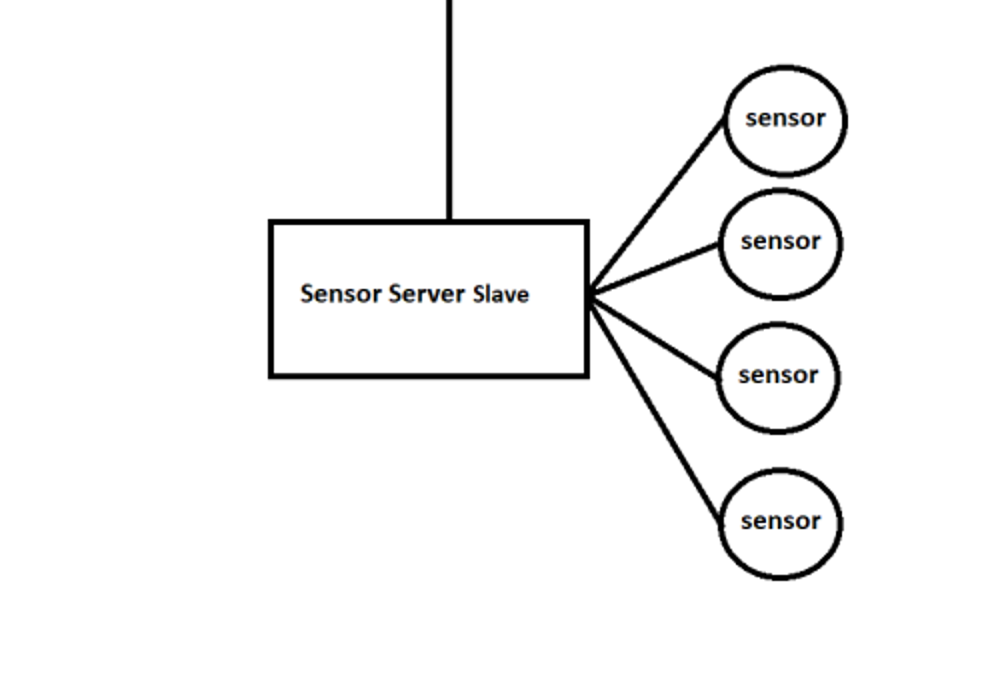
\includegraphics[width=\linewidth,height=.72\textheight,keepaspectratio]{assets/018_p002_01_panel2.png}\caption{Diagram or recorded result: Part 2: two-layer storage and caching, 20 percent. Panel 2 of 2.}\label{fig:018_p002_011}\end{figure}
\clearpage
\section{Part 3: MQTT gateway, 15 percent}

Connect the preceding API to MQTT. Version 3.1.1 or 5 is allowed;\allowbreak{} identify the chosen version, QoS, and reasons. Run a broker such as Mosquitto. Design and explain request and response topics, publication, subscription, and sensor-read message formats. Write a two-round sensor-call script, measure both round times, and compare them. Submit integration code, Makefile, build/\allowbreak{}run script, MQTT configuration, test script, installation/\allowbreak{}configuration guide, and a diagram showing API, broker, master, and slaves. The guide must explain installation, configuration, topics, application startup, mosquitto\_\allowbreak{}pub requests, mosquitto\_\allowbreak{}sub responses, test execution, and timing. Distinguish internal processing time from full client request/\allowbreak{}response time when analyzing caching.

\section{Part 4: SNMP sensor access, 15 percent}

Research SNMP and its monitoring role;\allowbreak{} a short report is required. Use snmpd to expose sensor data. Define custom OIDs. For each sensor, expose at least its name, description, and latest stored value. Use snmpwalk and provide a script that reads all sensors. Configure custom OIDs with snmpd's pass facility. Submit SNMP configuration, custom-OID adapter, all-sensor read script, Makefile where compilation is required, build/\allowbreak{}run script, and a guide to installation, configuration, and tests. Explain SNMP, OID, MIB, and the acquisition path. The guide must cover package installation, snmpd configuration, OID structure, service startup, snmpwalk use, test script, and the flow from database to SNMP response.

\section{Part 5: dated sensor history API, 5 percent}

Implement a Mongoose API in C/\allowbreak{}C+\allowbreak{}+\allowbreak{} accepting sensor name, identifier, and a date. Read and return that sensor's values on the specified date from the database in a consistent, readable response. Return a meaningful no-data message when appropriate. Supply Makefile, Bash build/\allowbreak{}run script, optional database initialization, and Markdown execution/\allowbreak{}test instructions. The assignment's example requests temperature sensor 101 on 2026-06-01. Its response contains sensor\_\allowbreak{}name, sensor\_\allowbreak{}id, date, and a values array, with examples 10:\allowbreak{}15:\allowbreak{}00 -> 24.8 and 10:\allowbreak{}30:\allowbreak{}00 -> 25.1. Preserve this as an example contract, not as a hard-coded result. The report must explain request and response formats and the database-reading path.

\section{Part 6: persistent alert daemon, 5 percent}

Write a background daemon that periodically checks sensor readings and inserts alert events into a database when configured conditions are met. Define the rules and record sensor identifier, sensor name/\allowbreak{}type, observed value, alert type, time, and status. Include a systemd service, Makefile, Bash build/\allowbreak{}run script, and installation/\allowbreak{}start/\allowbreak{}stop/\allowbreak{}status guide. Example rules include excessive temperature, humidity outside a permitted range, no data within a timeout, and physically invalid readings. The proposed alerts schema contains id INTEGER PRIMARY KEY AUTOINCREMENT, sensor\_\allowbreak{}id TEXT, sensor\_\allowbreak{}name TEXT, alert\_\allowbreak{}type TEXT, sensor\_\allowbreak{}value TEXT, created\_\allowbreak{}at TEXT, and status TEXT. Explain the daemon's diagram, decision logic, and persistent storage. Submit source, Makefile, service, installation/\allowbreak{}start script, alert-table initializer, guide, and report. The daemon guide must show compilation;\allowbreak{} service installation;\allowbreak{} starting, stopping, and status inspection;\allowbreak{} system logs;\allowbreak{} database inspection;\allowbreak{} and exact alert rules.

\section{Report and final-delivery checklist}

For every part, describe architecture, components, interconnections, request/\allowbreak{}response flow, storage, errors, dynamic IP/\allowbreak{}port management, relevant security analysis, cache/\allowbreak{}MQTT timing, and a diagram. Verify that all six independent directories have Markdown guides, Makefiles, build/\allowbreak{}run scripts, initialization and test scripts, diagrams, test outputs, and explanations. Programs must accept changed evaluation data and use only C/\allowbreak{}C+\allowbreak{}+\allowbreak{}.

\end{document}